\newpage
\appendix
\chapter{Appendix}

\begin{figure}
    \centering
    \begin{subfigure}[b]{\textwidth}
        
\includegraphics[width=\textwidth]{fig/PCA/pca0}
        \caption{First Principal Component}
    \end{subfigure}
    \begin{subfigure}[b]{\textwidth}
        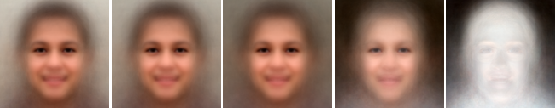
\includegraphics[width=\textwidth]{fig/PCA/pca1}
        \caption{Second Principal Component}
    \end{subfigure}
    \begin{subfigure}[b]{\textwidth}
        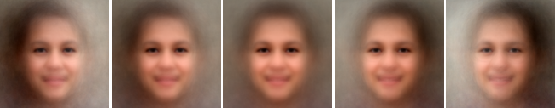
\includegraphics[width=\textwidth]{fig/PCA/pca2}
        \caption{Third Principal Component}
    \end{subfigure}
    \begin{subfigure}[b]{\textwidth}
        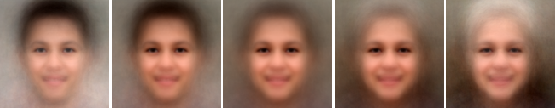
\includegraphics[width=\textwidth]{fig/PCA/pca3}
        \caption{Fourth Principal Component}
    \end{subfigure}
    \begin{subfigure}[b]{\textwidth}
        
\includegraphics[width=\textwidth]{fig/PCA/pca4}
        \caption{Fifth Principal Component}
    \end{subfigure}
    \begin{subfigure}[b]{\textwidth}
        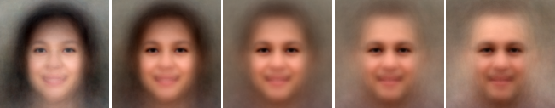
\includegraphics[width=\textwidth]{fig/PCA/pca5}
        \caption{Sixth Principal Component}
    \end{subfigure}
    \caption{Synthetic faces created by varying a single principal component to the mean face.}
    \label{pca-components}
\end{figure}

\begin{figure}
    \centering
    \begin{subfigure}[b]{0.45\textwidth}
        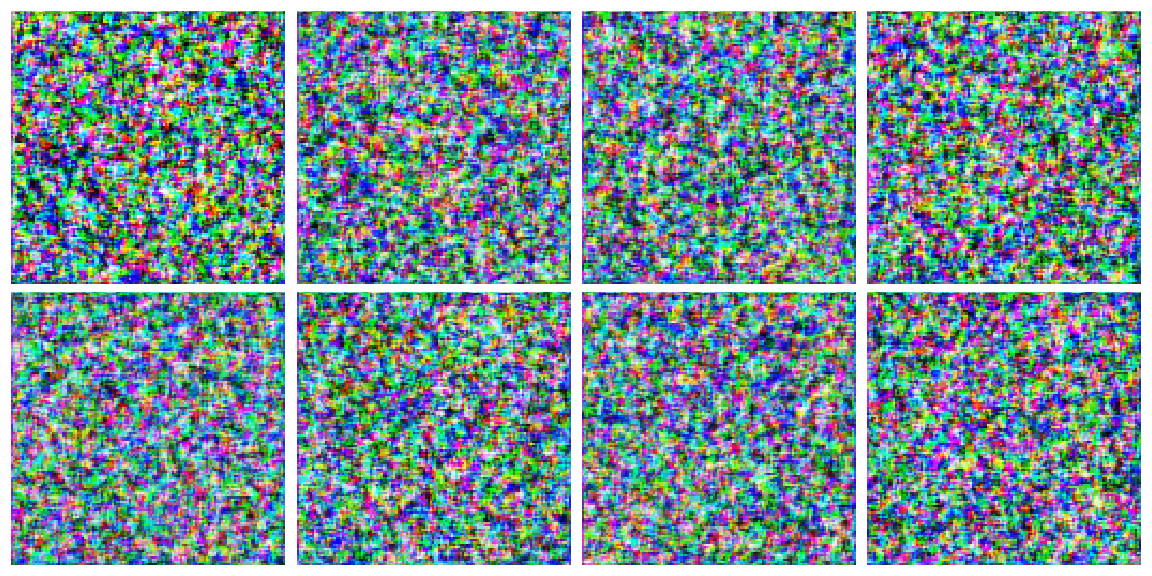
\includegraphics[width=\textwidth]{fig/dcgan/ffhq/epoch0}
        \caption{Epoch 0}
    \end{subfigure}
    ~
    \begin{subfigure}[b]{0.45\textwidth}
        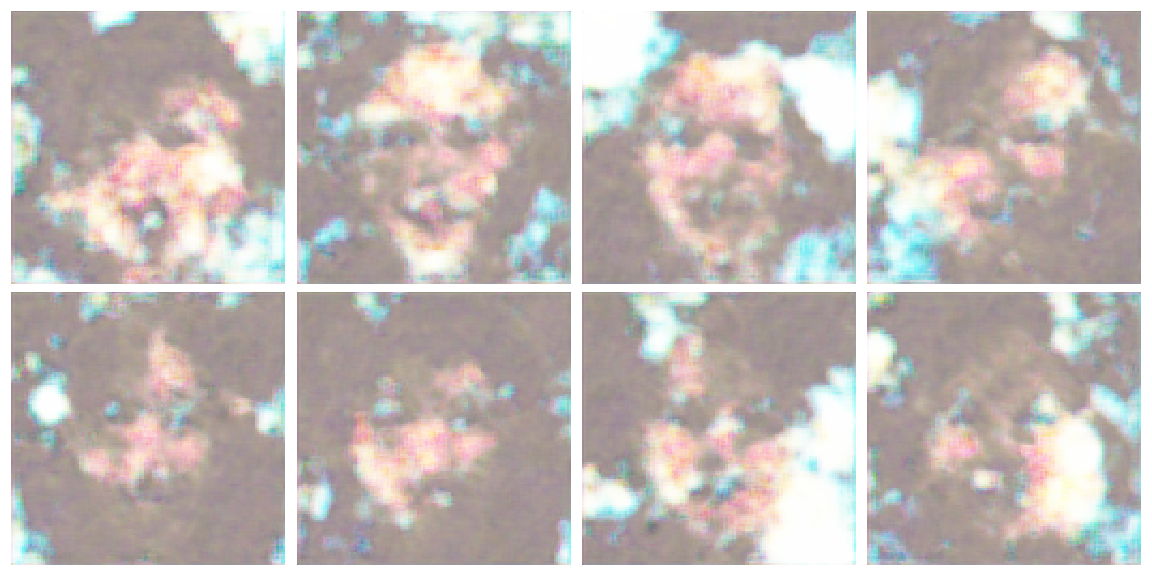
\includegraphics[width=\textwidth]{fig/dcgan/ffhq/epoch200}
        \caption{Epoch 10}
    \end{subfigure}

    \begin{subfigure}[b]{0.45\textwidth}
        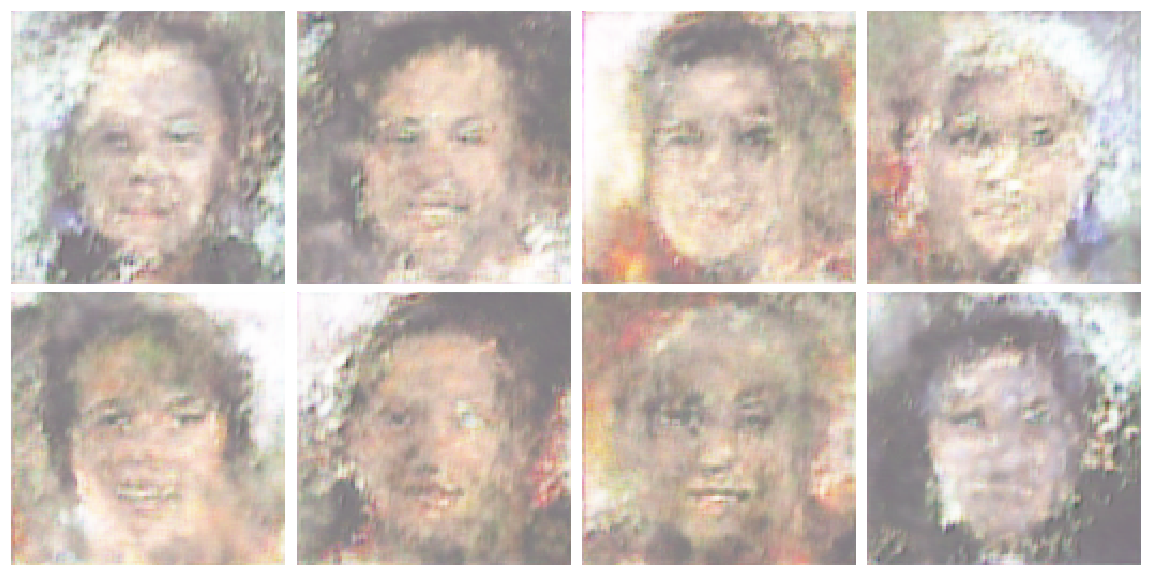
\includegraphics[width=\textwidth]{fig/dcgan/ffhq/epoch2000}
        \caption{Epoch 200}
    \end{subfigure}
    ~
    \begin{subfigure}[b]{0.45\textwidth}
        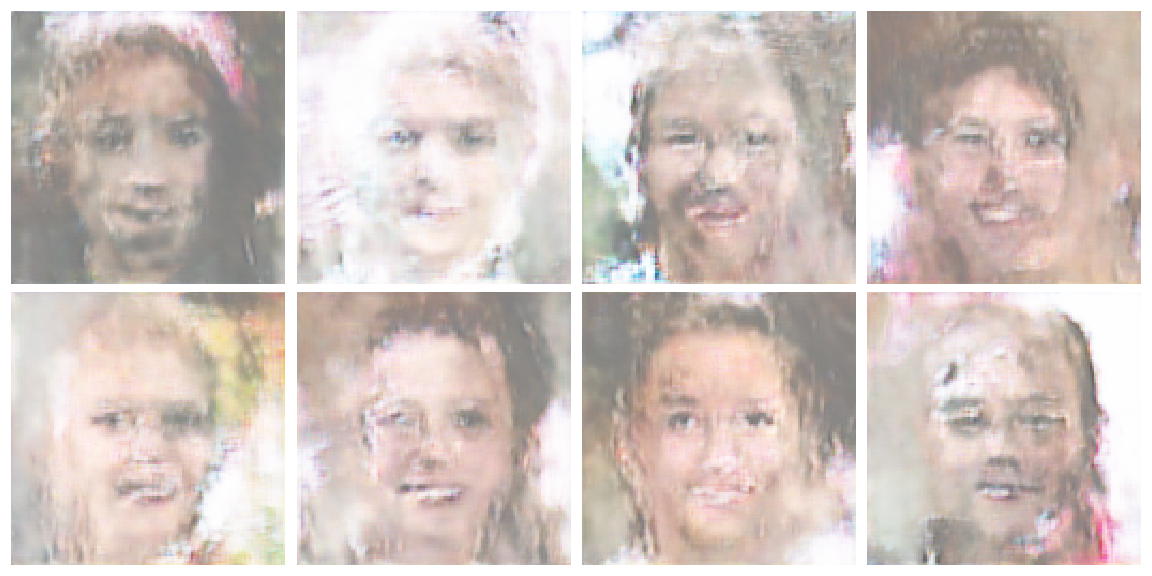
\includegraphics[width=\textwidth]{fig/dcgan/ffhq/epoch4000}
        \caption{Epoch 400}
    \end{subfigure}

    \begin{subfigure}[b]{\textwidth}
        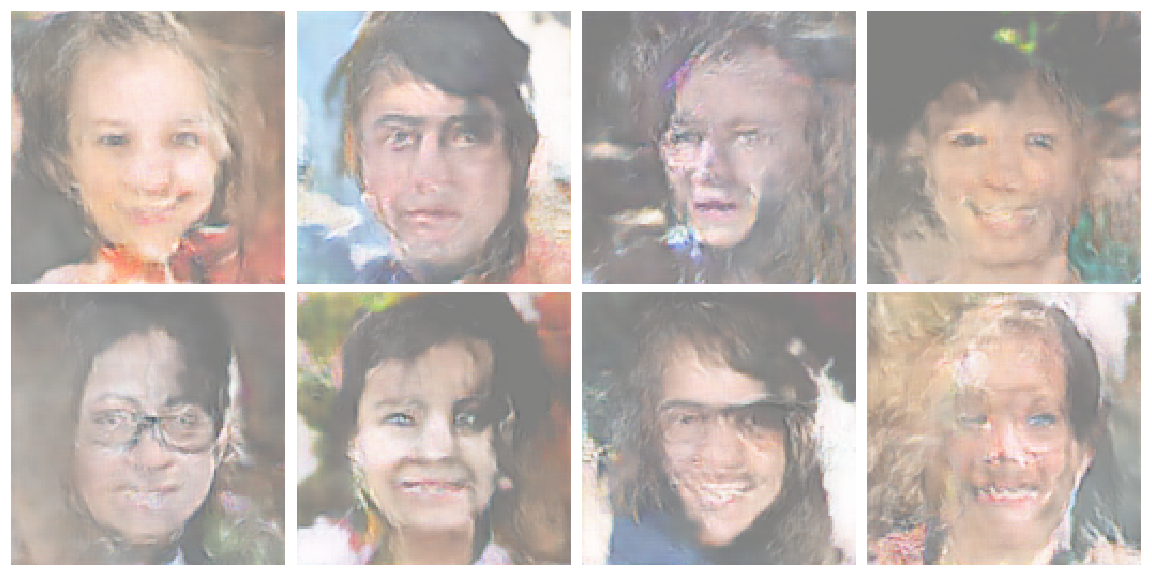
\includegraphics[width=\textwidth]{fig/dcgan/ffhq/epoch10000}
        \caption{Epoch 400}
    \end{subfigure}
    \caption{Samples from DCGAN during training on the FFHQ dataset}
    \label{dcgan-ffhq-samples}
\end{figure}


\begin{figure}

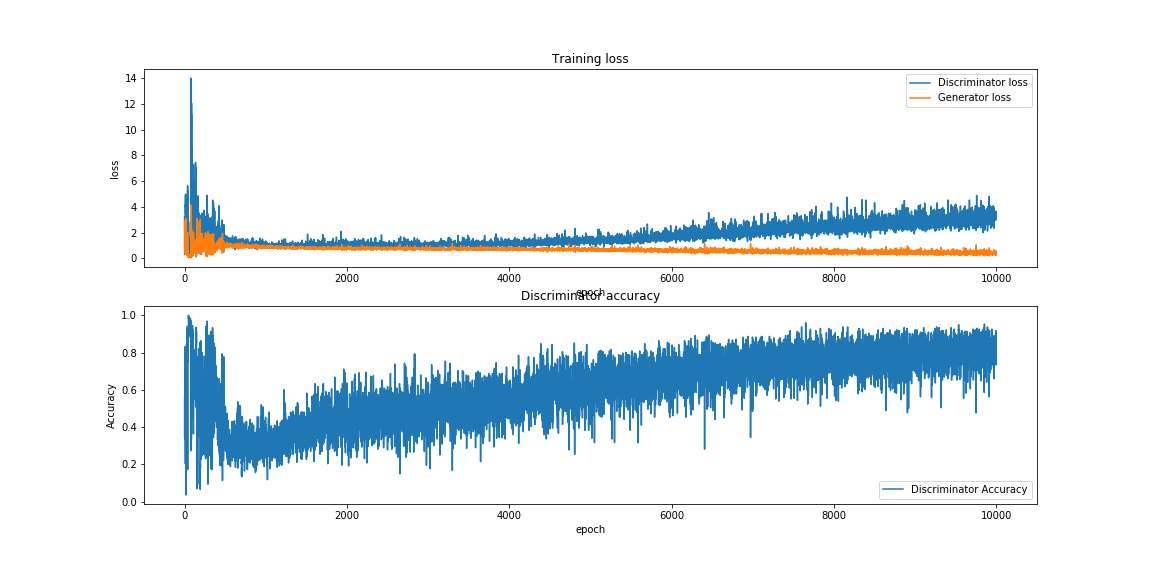
\includegraphics[width=\textwidth]{fig/dcgan/ffhq/loss}
  \caption{Loss and accuracy of the discriminator during training on the FFHQ Datase}
  \label{dcgan-ffhq-loss}
\end{figure}

\begin{figure}
    \centering
    \begin{subfigure}[b]{0.45\textwidth}
        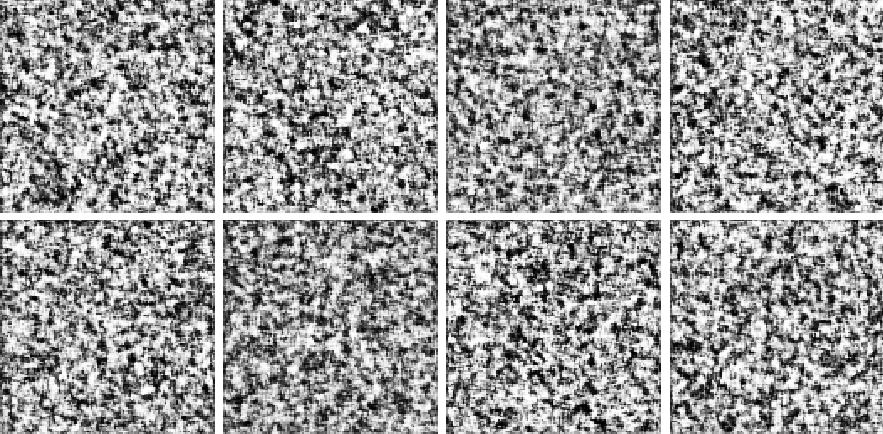
\includegraphics[width=\textwidth]{fig/dcgan/caltech/epoch0}
        \caption{Epoch 0}
    \end{subfigure}
    ~
    \begin{subfigure}[b]{0.45\textwidth}
        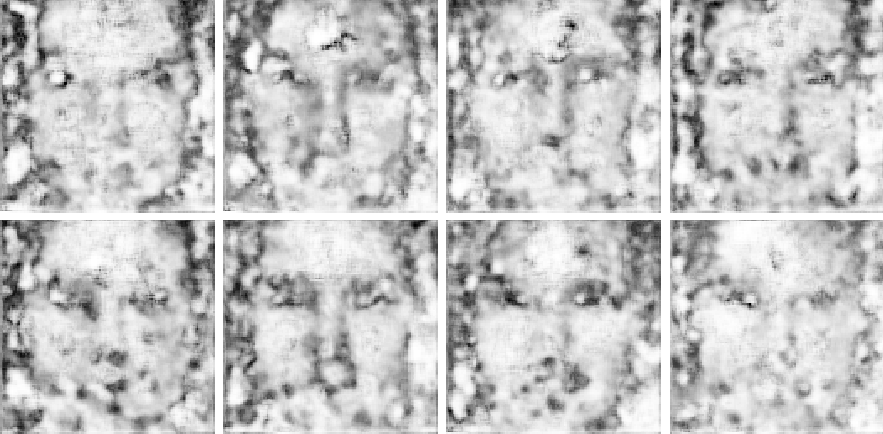
\includegraphics[width=\textwidth]{fig/dcgan/caltech/epoch200}
        \caption{Epoch 10}
    \end{subfigure}

    \begin{subfigure}[b]{0.45\textwidth}
        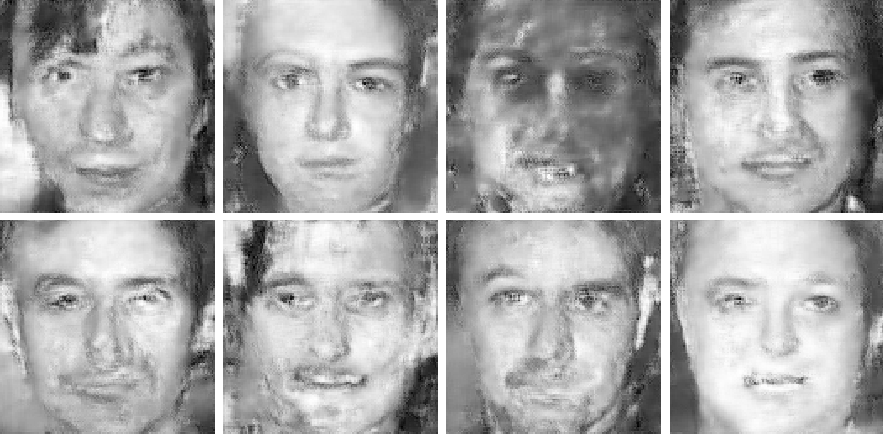
\includegraphics[width=\textwidth]{fig/dcgan/caltech/epoch2000}
        \caption{Epoch 200}
    \end{subfigure}
    ~
    \begin{subfigure}[b]{0.45\textwidth}
        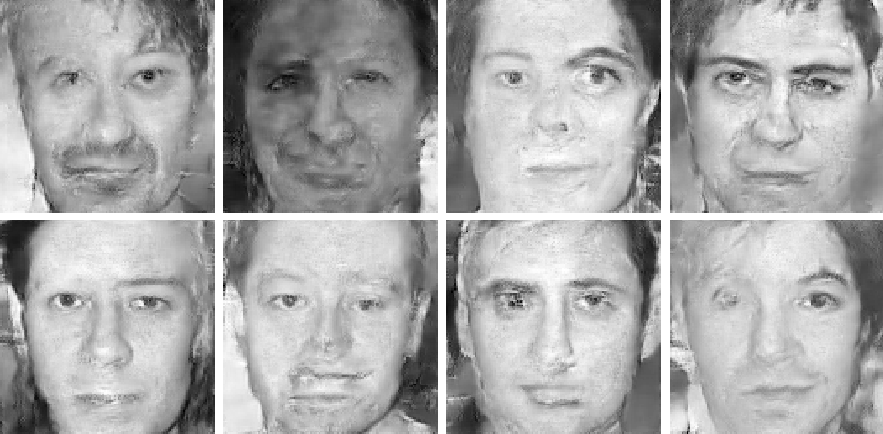
\includegraphics[width=\textwidth]{fig/dcgan/caltech/epoch4000}
        \caption{Epoch 400}
    \end{subfigure}

    \begin{subfigure}[b]{\textwidth}
        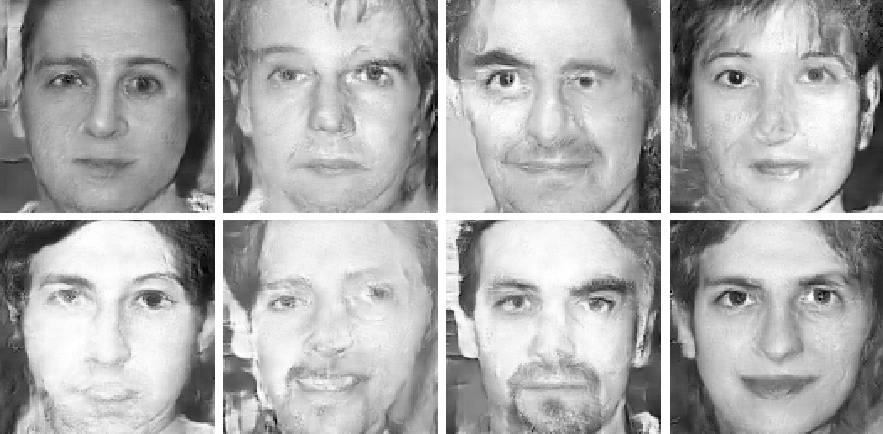
\includegraphics[width=\textwidth]{fig/dcgan/caltech/epoch10000}
        \caption{Epoch 400}
    \end{subfigure}
    \caption{Samples from DCGAN during training on the Caltech dataset}
    \label{dcgan-caltech-samples}
\end{figure}

\begin{figure}

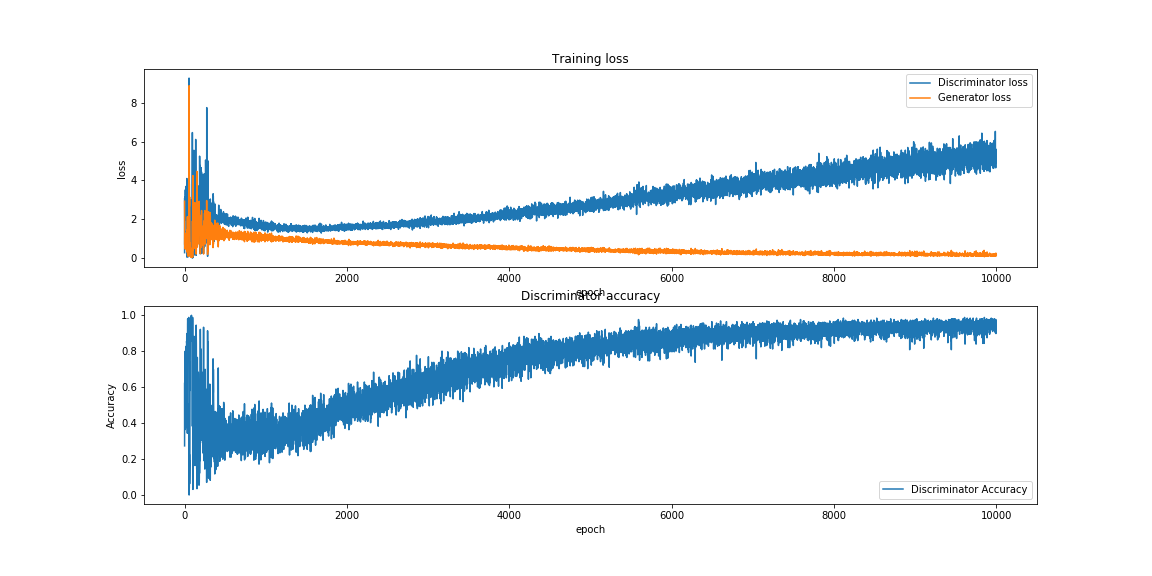
\includegraphics[width=\textwidth]{fig/dcgan/caltech/loss}
  \caption{Loss and accuracy of the discriminator during training on the Caltech Dataset}
  \label{dcgan-caltech-loss}
\end{figure}
